
\begin{figure}[h!]
    \centering
    \caption{Estimates of the effect of the MW on rents, county by month data}
    \label{fig:dynamic_stacked}

	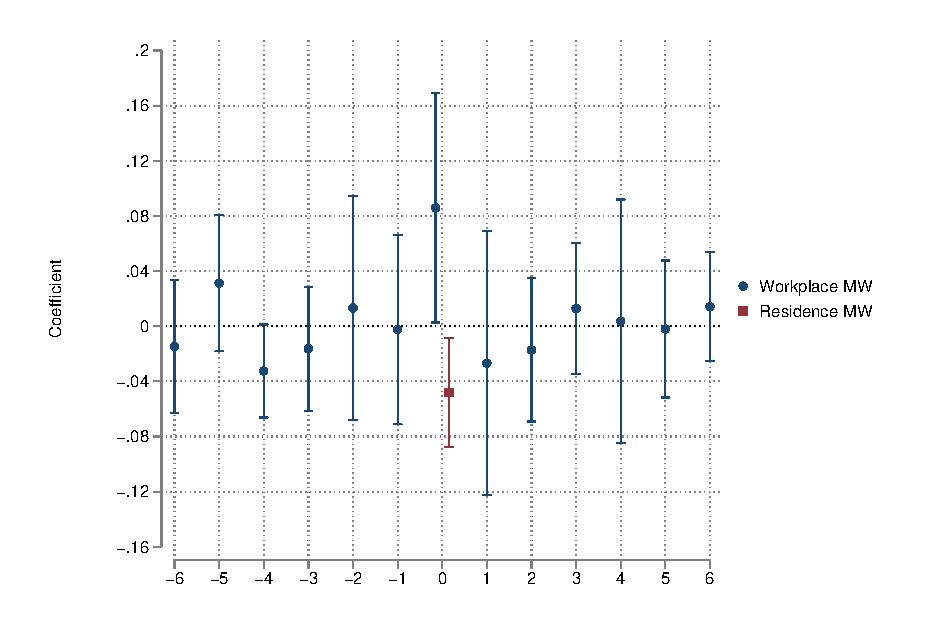
\includegraphics[width = 0.75\textwidth]{fd_stacked/output/fd_mw_wkp_only_dynamic_w6.eps}

    \begin{minipage}{.95\textwidth} \footnotesize
        \vspace{3mm}
        Notes:
        Data are from Zillow \parencite{ZillowData}, 
        the minimum wage panel described in Section \ref{sec:mw_construction}, 
        LODES origin-destination statistics \parencite{CensusLODES},
        and the QCEW \parencite{QCEW}.
        The figure mimics the estimates in Figure \ref{fig:dynamic_baseline} using a 
        ``stacked'' sample.
        To construct the sample we proceed as follows.
        First, we define a CBSA-month as treated if in that month there is at 
        least one ZIP code that had a change in the binding MW.
        We drop events that have less than 10 ZIP codes.
        For each of the selected CBSA-months we assign a unique event ID. 
        Second, for each event we take a window $w = 6$, and we keep all months 
        within that window for the ZIP codes that belong to the treated CBSA.
        If a ZIP code has missing data for some month within the window, we drop 
        the entire ZIP code from the respective event.
        We plot coefficients from regressions of the log of rents per
        square foot on the residence and workplace MW measures, including 
        six leads and lags of the workplace MW measure.
        All regressions are estimated in first differences and include 
        time-period fixed effects and economic controls that vary at the 
        county and month levels.
        The measure of rents per square foot corresponds to the Single Family, 
        Condominium and Cooperative houses from Zillow.
        The residence MW is defined as the log statutory MW at the County.
        The workplace MW is defined as the log statutory MW where the average 
        resident of the county works, constructed using LODES 
        origin-destination data.
        Economic controls from the QCEW include the change of the following 
        variables: the log of the average wage, the log of employment, and the 
        log of the establishment count for the sectors ``Information,'' 
        ``Financial activities,'' and ``Professional and business services.''
        95\% pointwise confidence intervals are obtained from standard errors 
        clustered at the state level.
    \end{minipage}
\end{figure}
